\chapter{Экспериментальная проверка Алгоритмов геолокации}

\section{Состав и структура реализованного программного обеспечения}

\section{Описание обучающих и тестовых данных}

Для тестирования разработанной системы использовались снимки \texttt{Google Street View} из 10 городов снятые в панорамном режиме с разрешением $ 224\times224 $. Код, генерирующий эти снимки представлен на листинге \ref{lst:Gen}.

Так как \texttt{API Google Street View} отвечает картинкой и не для всех координат в городе существуют панорамы, отфильтровывать ошибки можно просто используя размер картинки
как хэш функцию. Коллизии маловероятны из-за того что обычно панорамы на порядок отличаются по размеру от картинки, обозначающей ошибку. Интересующая нас часть листинга представлена ниже.

\begin{lstlisting}[language=python, float=tb,frame=lines,label=lst:frag1]
# check if the downloaded image was invalid and if so remove it
...
if os.path.isfile(filepath):
	size = os.path.getsize(filepath)
	if size == FAILED_DOWNLOAD_IMAGE_SIZE:
		os.remove(filepath)
		misses += 1
	else:
		num_imgs += 1
...
\end{lstlisting}

Снимки генерируются методом случайного сдвига точки к которой делается запрос и случайного поворота.

Для разделения на тестовую и обучающую выборки также используются скрипты.

\section{Результаты экспериментов}

\subsection{Эксперимент с 1 изображением}

Было проведено обучение модели на основе свёрточной сети \texttt{resnet34} с использованием подхода \texttt{transfer learning}. Для оптимизации использовался 
метод Стохастического градиентного спуска с параметрами $ \mbox{скорость обучения} = 0,001 и \mbox{momentum} = 0.9$. В процессе обучения каждые 7 шагов скорость обучения 
сокращалась в 10 раз. Гиперпараметры подобраны методом поиска по решетке со скользящим контролем. Для этого использовался метод \texttt{sklearn.model\_selection.GridSearchCV}

В качестве функции потерь использовалась <<Перекрёстная энтропия>>.
На листинге ниже представлены определения для обучения сети.
Процедура обучения сети описана в листинге \ref{lst:Training}
\begin{lstlisting}[language=python,frame=lines]
model_ft = models.resnet34(pretrained=True)
num_ftrs = model_ft.fc.in_features
model_ft.fc = nn.Linear(num_ftrs, len(class_names))

model_ft = model_ft.to(device)

criterion = nn.CrossEntropyLoss()

# Observe that the last layer parameters are being optimized
optimizer_ft = optim.SGD(model_ft.fc.parameters(), lr=0.001, momentum=0.9)

# Decay LR by a factor of 0.1 every 7 epochs
exp_lr_scheduler = lr_scheduler.StepLR(optimizer_ft, step_size=7, gamma=0.1)

\end{lstlisting}

Для варианта с переобучением последнего слоя:
 
Обучение проходило 40 эпох. Время обучения --- $ \approx 5 $ мин.

\texttt{F1}-взвешенная оценка для классификации $ 0.5101 $
Результаты классификации представлены на иллюстрациях и в таблице \ref{tbl:acc}.

Для варианта с переобучением всей сети:

Обучение проходило 30 эпох. Время обучения --- $ \approx9 $ мин.

\texttt{F1}-взвешенная оценка для классификации $ 0.50 $
Результаты классификации представлены на иллюстрациях и в таблице \ref{tbl:acc2}.

В сравнении с другими архитектурами resNet34 выиграл по времени обучения у resNet50, Inception\_V3, DenseNet и по качеству классификации у squeezeNet.

\begin{figure}
	\centering
	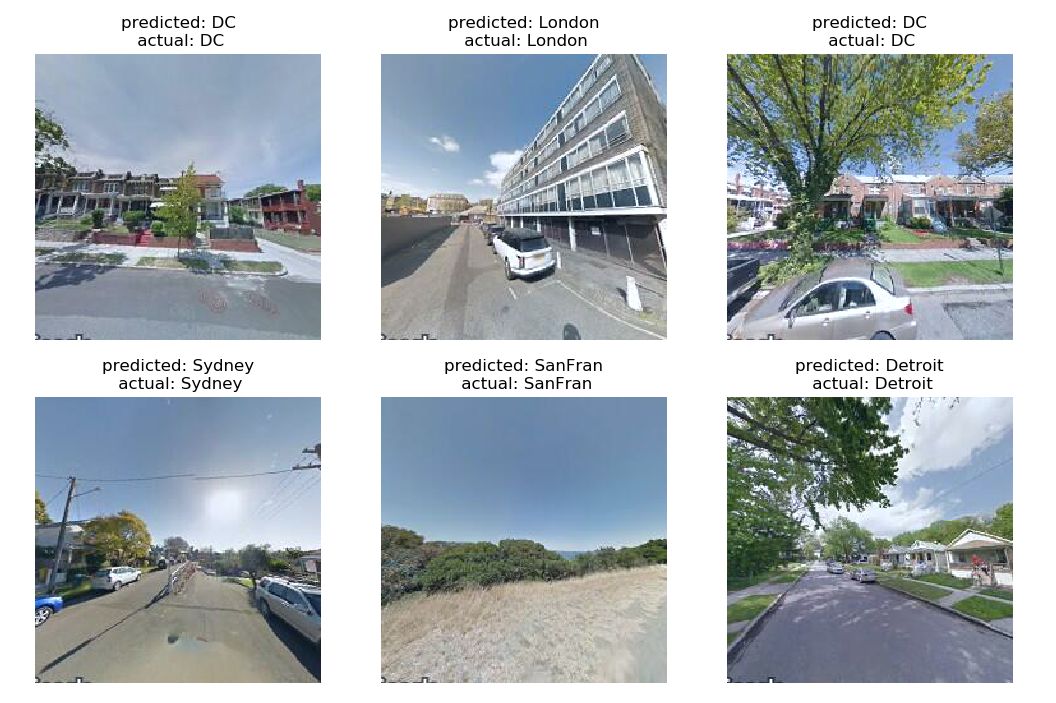
\includegraphics[width=0.9\linewidth]{img/res1im}
	\caption{Результат обучения модели с resNet18 по 1 изображению. \\
			 Пример удачно выпавших классов}
	\label{fig:res1im}
\end{figure}
\begin{figure}[h]
	\centering
\begin{subfigure}{0.4\linewidth}
	\centering
	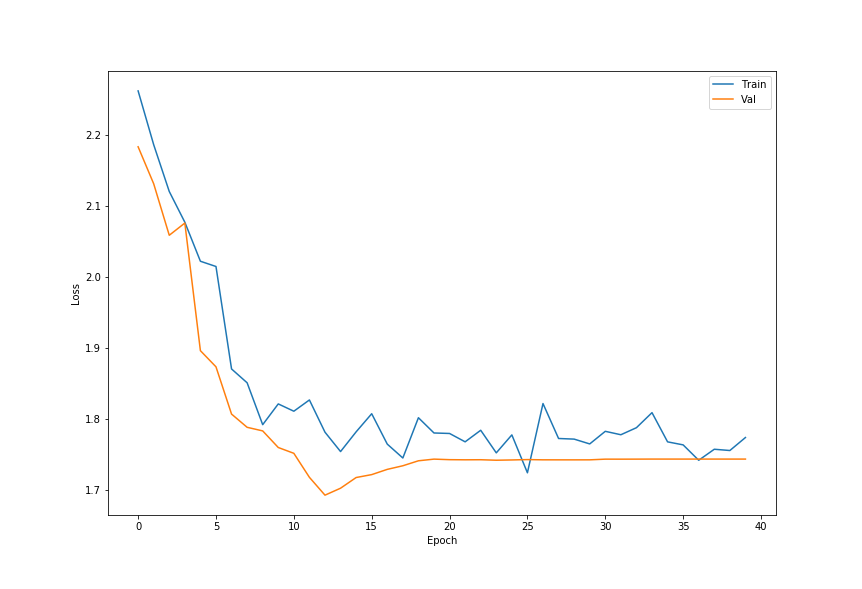
\includegraphics[width=0.9\linewidth]{img/train1im}
	\caption{ для варианта с переобучением последнего слоя}
	\label{fig:train1im}
\end{subfigure}
\begin{subfigure}{0.4\linewidth}
	\centering
	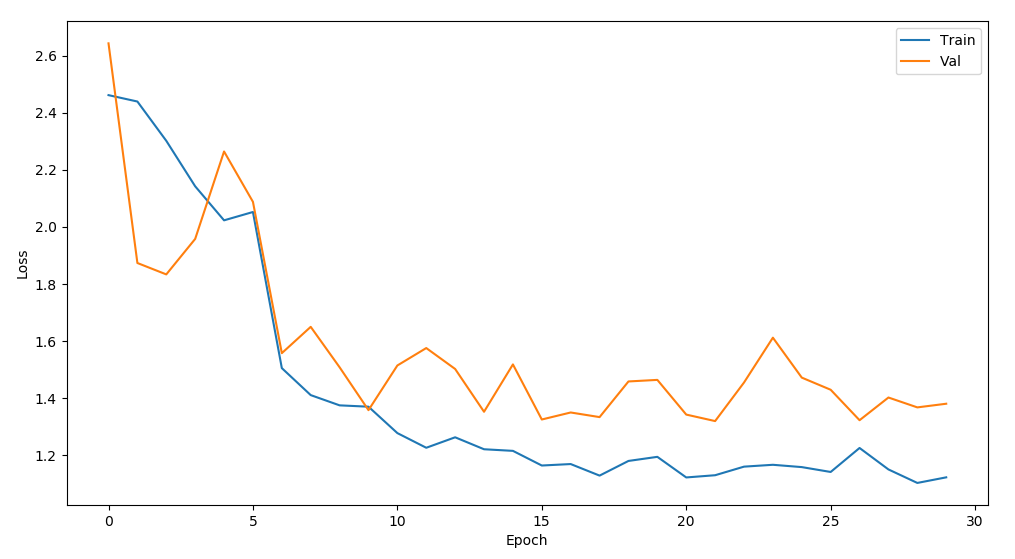
\includegraphics[width=1\linewidth]{img/train1im2}
	\caption{при дообучении всех слоёв сети.}
	\label{fig:train1imretr}
\end{subfigure}
\caption{Значение функции потерь на Обучающей и Валидационной выборках по эпохам }
\end{figure}

\begin{table}
	\parbox{.45\linewidth}{
	\begin{tabu} {l|c}
		Выборка   & Точность распознавания \\ \hline
		Обучение  &         0.711          \\
		Валидация &         0.424          \\
		Тест      &         0.602          \\ \hline
	\end{tabu}
	\caption{Точность распознавания для архитектуры \texttt{resnet34} c переобучением всех слоёв}
	\label{tbl:acc}
}\hfill
\parbox{.45\linewidth}{
	\begin{tabu} {l|c}
		Выборка   & Точность распознавания \\ \hline
		Обучение  &         0.421          \\
		Тест      &         0.429          \\
		Валидация &         0.384          \\ \hline
	\end{tabu}
	\caption{Точность распознавания для архитектуры \texttt{resnet34} c переобучением последнего слоя}
	\label{tbl:acc2}

}
\end{table}

\subsection{Эксперимент с альбомом} 

Мы сравниваем эту модель с моделью и базовый уровень, который просто усредняет прогнозы по одному изображению всех изображений в альбоме и назначает
среднее для всех изображений. Усреднение в альбомах ($ \mathcal{G}= \mathbb{E}[ \mathcal{F}(X) ] $) уже дают значительное улучшение по сравнению с одним изображением
(45,7\% на уровне улиц), поскольку у него больше
вмятины предсказания к неоднозначным изображениям. Однако, LSTM
модель явно превосходит технику усреднения (50,5\%
относительное улучшение уровня улицы). Визуальный контроль
результатов показали, что за достоверностью следуют несколько изображений с более низким местоположением уверенность, модель LSTM присваивает низкий уровень доверия изображения, расположенные вблизи изображения с высокой степенью достоверности в то время как $ \mathcal{F} $ может «прыгать» (менять предположение о расположении альбома), модель LSTM имеет тенденцию прогнозировать близкие местоположения, кроме случаев когда есть убедительные доказательства изменения местоположения. LSTM модель работает лучше усреднения из-за того что оно присваивает всем изображениям в альбоме одинаковые уровни значимости и не может производить точные прогнозы для альбомов которые включают разные местоположения (например, альбомы поездок).

\section{Сравнение реализованного программного обеспечения с существующими аналогами}

В качестве аналогов выступают системы PlaNet и Im2GPS.
Для сравнения будем использовать оценку точности на уровне 
региона ( 750 км ), так как континентов $ \approx 6 $ а регионов несколько больше.

\begin{table}[h]
\centering
\begin{tabu}{c|c}

Система	& Точность \\ \hline
PlaNet	& 53.6\% \\  
IM2GPS	& 35.4\% \\  
\textbf{Разрабатываемая система}& \textbf{44.7}\%  \\ \hline 
\end{tabu}
\caption{Сравнение показателей точности} 
\end{table}

\section{Выводы}

Были разработаны скрипты для генерации <<датасета>>, разбиения на  обучающую / тестовую / валидационную, приведения датасета к читаемому виду. Также были исследованы методы \texttt{transfer learning}, был произведён их сравнительный анализ и была выявлена следующая закономерность: дообучение последнего слоя не уступает по качеству переобучению всей сети, несмотря на более высокие показатели качества на тестовой выборке.

Было проведено сравнение с более ранними разработками и достигнут уровень точности
сопоставимый с ними.
